\section{1174040 - Hagan Rowlenstino A. S}
    \subsection{Teori}
        \begin{enumerate}
            \item Jelaskan Apa Itu binari calssification dilengkapi ilustrasi gambar sendiri.\par
            Binary Classification adalah sebuah aksi dimana dilakukannya klasifikasi dari sebuah kumpulan objek tertentu ke dalam dua buah kelompok yang berbeda berdasarkan beberapa fitur atau sifat-sifat.
            \begin{figure}[H]
                \includegraphics[width=4cm]{figures/1174040/chapter2/binary.jpeg}
                \centering
                \caption{Binary Classification}
            \end{figure}
            
            \item Jelaskan Apaitu supervised learning , unsupervised learning dan clusterring dengan ilustrasi gambar sendiri.\par
            Supervised learning adalah sebuah cara untuk mengklasifikasikan kumpulan objek yang fitur ataupun sifat-sifatnya dari kelas nya sudah di tentukan sebelumnya. contoh pada merk mobil honda yang merupakan buatan jepang dan ferarri merupakan buatan eropa\par
            \begin{figure}[H]
                \includegraphics[width=4cm]{figures/1174040/chapter2/supervised.jpeg}
                \centering
                \caption{Supervised}
            \end{figure}

            Unsupervised learning merupakan teknik pengklasifikasian tanpa perlu di supervised sebelumnya, dimana model tersebut yang akan bekerja sendiri untuk menemukan infomasi yang terkait. seperti pada contoh di gambar.\par
            \begin{figure}[H]
                \includegraphics[width=4cm]{figures/1174040/chapter2/unsupervised.jpeg}
                \centering
                \caption{Unsupervised}
            \end{figure}

            clustering merupakan metode pengelompokan data dengan membagi ke dalam beberapa kelompok. disini saya memberi contoh dengan kriteria kendaraan yang lebih dari 2,1 ton dan kurang dari 2,1 ton.\par
            \begin{figure}[H]
                \includegraphics[width=4cm]{figures/1174040/chapter2/cluster.jpeg}
                \centering
                \caption{lustering}
            \end{figure}

            \item Jelaskan apa itu evaluasi dan akurasi dan disertai ilustrasi contoh dengan gambar sendiri.\par
            Evaluasi adalah proses yang sistematis yang ditujukan untuk menentukan ataupun membuat keputusan dengan memeriksa pernyataan-pernyataan yang telah ada sebelumnya.Akurasi adalah tingkat ketepatan dari sebuah data yang telah di hasilkan dari evaluasi yang telah dilakukan sebelumnya.
            \begin{figure}[H]
                \includegraphics[width=4cm]{figures/1174040/chapter2/evaluasi.jpeg}
                \centering
                \caption{Evaluasi}
            \end{figure}

            \item Jelaskan bagaimana cara membuat Confusion Matrix, Buat confusion matrix sendiri.\par
            Untuk membuat confusion matrix kita perlu menentukan objek yang akan dievaluasi terlebih dahulu, setelah itu tentukan nilai miring pada setiap kolom objek tersebut lalu setiap baris dan jika nlainya di bagi baris dan kolom nya, harus bernilai sesuai nilai yang telah di tetapkan sebelumnya.
            \begin{figure}[H]
                \includegraphics[width=4cm]{figures/1174040/chapter2/confused.jpeg}
                \centering
                \caption{Confussion Matrix}
            \end{figure}

            \item Jelaskan bagaimana K-fold cross validation bekerja dengan gambar ilustrasi contoh buatan sendiri.\par
            Melatih mesin dengan membagi data set yang akan di olah menjadi dua buah yaitu data testing dan training. sebagai contoh ada 500 data pada dataset, maka 200 sebagai data testing dan 300 akan menjadi data training.
            \begin{figure}[H]
                \includegraphics[width=4cm]{figures/1174040/chapter2/k.jpeg}
                \centering
                \caption{K-Fold}
            \end{figure}

            \item Jelaskan Apa itu decision tree dengan gambar ilustrasi contoh buatan sendiri.\par
            Desicsion tree adalah sebuah model prediksi yang menggunakan struktur yang menyerupai pohon ataupun sebuah hirarki
            \begin{figure}[H]
                \includegraphics[width=4cm]{figures/1174040/chapter2/tree.jpeg}
                \centering
                \caption{Decision Tree}
            \end{figure}

            \item jelaskan apa itu information gain dan entropi dengan gambar ilustrasi buatan sendiri.\par
            information Gain mengukur berapa banyak informasi yang sebuah fitur berikan kepada kita tentang kelas tersebut. sedangkan entropi menentukan bagaimana decision tree memilah data nya.
            \begin{figure}[H]
                \includegraphics[width=4cm]{figures/1174040/chapter2/info.jpeg}
                \centering
                \caption{Information Gain}
            \end{figure}

        \end{enumerate}
    \subsection{scikit-learn}
        \begin{enumerate}
            \item  baris pertama yaitu mengimport library pandas. pada baris kedua ada funsi read\_csv untuk membaca file csv  serta datanya dipisah dengan tanda titik koma lalu dimasukkan kedalam variable bernama pisang. fungsi pada baris terakhir yaitu untuk mengetahui panjang data / banyak data yang ada\hfill \break \lstinputlisting[firstline=9, lastline=11]{src/1174040/chapter2/1174040.py}
            \begin{figure}[H]
                \includegraphics[width=4cm]{figures/1174040/chapter2/1.png}
                \centering
                \caption{No 1}
            \end{figure}

            \item Disini diginakan fungsi untuk menunjukkan lulus atau gagal dimana jika lulus ditanndai dengan angka 1 dan gagal dengan angka 0. data yang daka ndi cek yaitu data dari csv yang sebelumnya karena itu masih diigunakan variable pisang. yang selanjutnya akan dieksekusi.
            \hfill \break \lstinputlisting[firstline=15, lastline=18]{src/1174040/chapter2/1174040.py}
            \begin{figure}[H]
                \includegraphics[width=4cm]{figures/1174040/chapter2/2.png}
                \centering
                \caption{No 2}
            \end{figure}

            \item Disini yaitu mengkonversi kategori variable menjadi variable indikator
            \hfill \break \lstinputlisting[firstline=22, lastline=23]{src/1174040/chapter2/1174040.py}
            \begin{figure}[H]
                \includegraphics[width=4cm]{figures/1174040/chapter2/3.png}
                \centering
                \caption{No 3}
            \end{figure}

            \item bagian ini berfungsi untuk menentukan data training dan data testing dari dataset csv yang telah dimasukkan di dalam variable pisang tadi. lalu mengimport library numpy untuk operasi vektor serta matrix karena data diatas berupa matrix.
            \hfill \break \lstinputlisting[firstline=29, lastline=41]{src/1174040/chapter2/1174040.py}
            \begin{figure}[H]
                \includegraphics[width=4cm]{figures/1174040/chapter2/4.png}
                \centering
                \caption{No 4}
            \end{figure}

            \item pada baris pertam kita mengimport tree dari library sklearn yang berfunsi untuk membuat desicion tree
            \hfill \break \lstinputlisting[firstline=46, lastline=49]{src/1174040/chapter2/1174040.py}
            \begin{figure}[H]
                \includegraphics[width=4cm]{figures/1174040/chapter2/5.png}
                \centering
                \caption{No 5}
            \end{figure}

            \item mengimport library graphviz
            \hfill \break \lstinputlisting[firstline=54, lastline=59]{src/1174040/chapter2/1174040.py}

            \item untuk menyimpan data dari tree dan menarik data langsung dari desicion tree
            \hfill \break \lstinputlisting[firstline=64, lastline=65]{src/1174040/chapter2/1174040.py}
            \begin{figure}[H]
                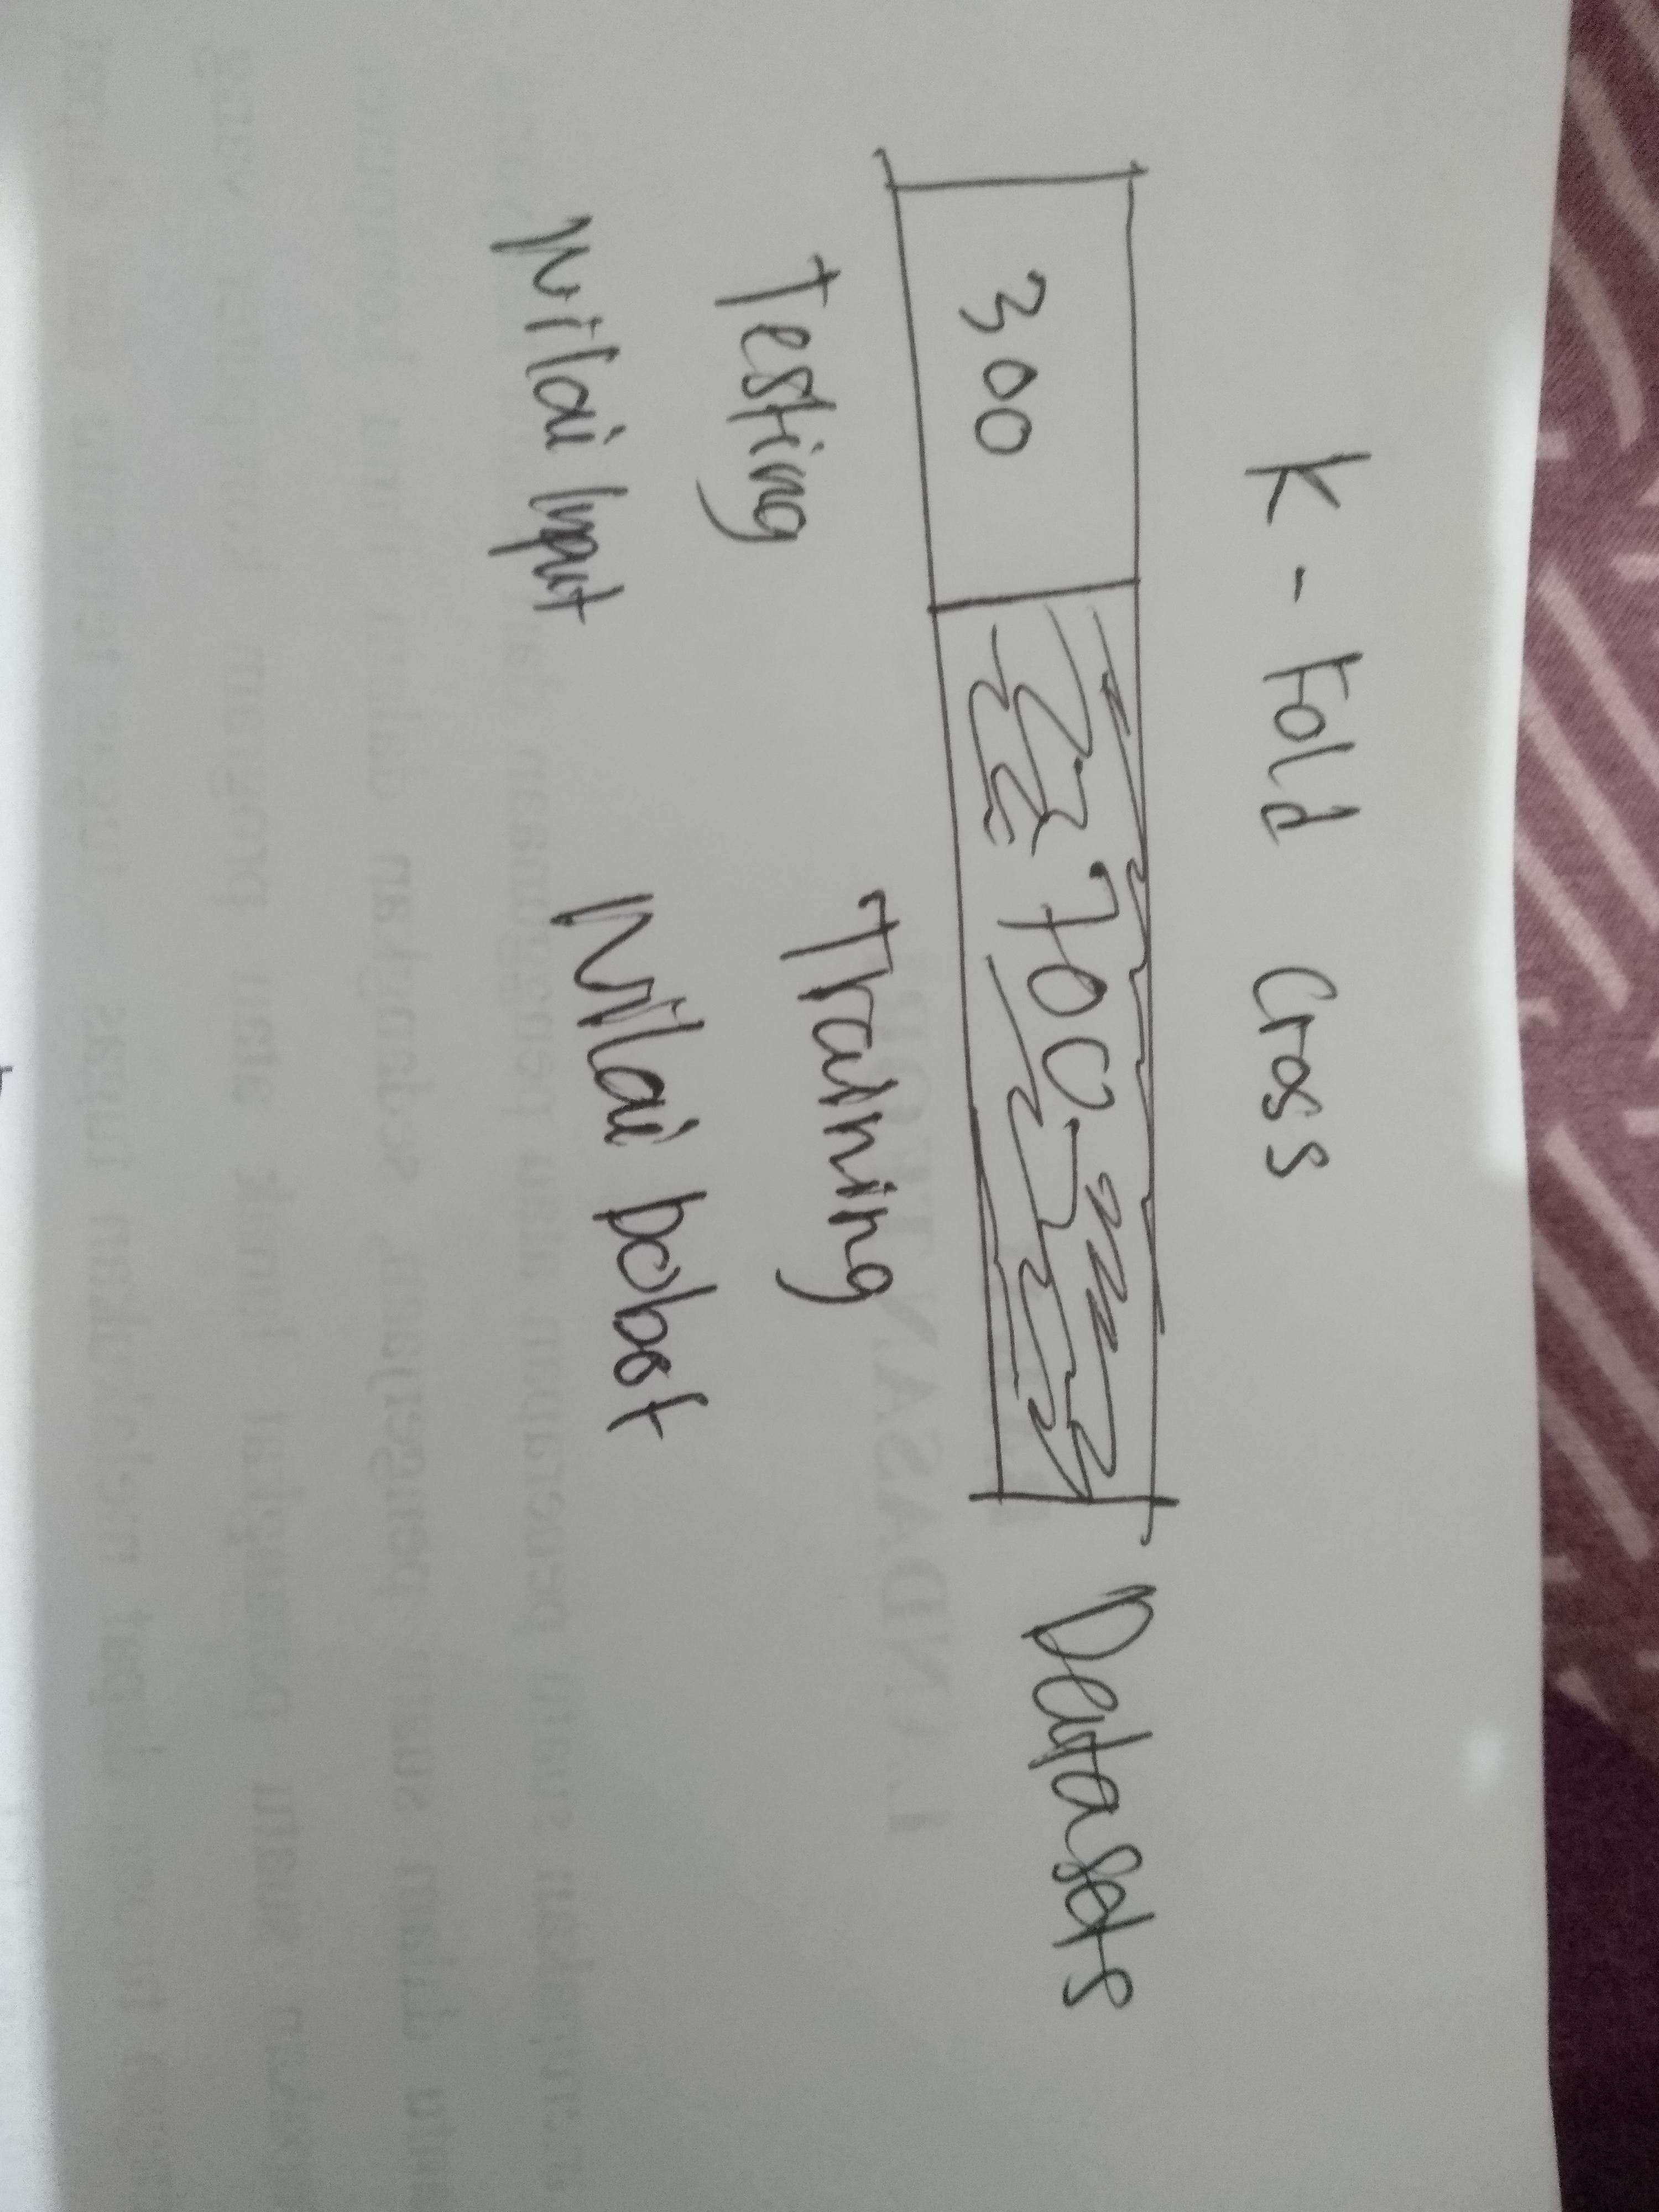
\includegraphics[width=4cm]{figures/1174040/chapter2/7.png}
                \centering
                \caption{No 7}
            \end{figure}

            \item untuk mencari ketepatan data yang telah diolah
            \hfill \break \lstinputlisting[firstline=69, lastline=69]{src/1174040/chapter2/1174040.py}

            \item untuk menghitung akurasi ketepatan data
            \hfill \break \lstinputlisting[firstline=73, lastline=77]{src/1174040/chapter2/1174040.py}
            \begin{figure}[H]
                \includegraphics[width=4cm]{figures/1174040/chapter2/9.png}
                \centering
                \caption{No 9}
            \end{figure}

            \item membuat variable baru dengan nilai tree di dalamnya dengan bentuk akurasi yang spesifik
            \hfill \break \lstinputlisting[firstline=81, lastline=84]{src/1174040/chapter2/1174040.py}
            \begin{figure}[H]
                \includegraphics[width=4cm]{figures/1174040/chapter2/10.png}
                \centering
                \caption{No 10}
            \end{figure}

            \item menentukan rank batasannya yaitu 1 sampai 20 dari nilai tree tadi yang digunakan untuk menentukan nilai untuk grafik
            \hfill \break \lstinputlisting[firstline=88, lastline=98]{src/1174040/chapter2/1174040.py}
            \begin{figure}[H]
                \includegraphics[width=4cm]{figures/1174040/chapter2/11.png}
                \centering
                \caption{No 11}
            \end{figure}

            \item mengimport matplotlib.pyplot yang akan digunakan untuk membuat grafik
            \hfill \break \lstinputlisting[firstline=102, lastline=105]{src/1174040/chapter2/1174040.py}
            \begin{figure}[H]
                \includegraphics[width=4cm]{figures/1174040/chapter2/12.png}
                \centering
                \caption{No 12}
            \end{figure}
        \end{enumerate}
    \subsection{Penanganan Error}
        \begin{enumerate}
            \item Screenshot
            \begin{figure}[H]
                \includegraphics[width=4cm]{figures/1174040/chapter2/error.png}
                \centering
                \caption{Screenshot Error}
            \end{figure}
            \item Kode dan Jenis Error
            Jenis error adalah Key Error
            \hfill \break \lstinputlisting[firstline=22, lastline=23]{src/1174040/chapter2/err.py}
            \item Solusi Penanganan Error
            Mengganti kuda dengan pisang
        \end{enumerate}